\documentclass[aspectratio=169]{beamer}
\usetheme{Pittsburgh}
\usecolortheme{dove}
\usepackage{graphicx}
\usepackage[utf8]{inputenc}
\usepackage{amsmath}
\usepackage{amsfonts}
\usepackage{amssymb}
\usepackage{tikz}
\usetikzlibrary{3d, perspective, positioning, arrows.meta, calc, fadings, fit, backgrounds, shapes}
\usepackage[style=apa,backend=biber]{biblatex}
\addbibresource{/home/nicoluarte/Documents/repos/phd_DCCS/references/refs.bib}

\title{\textbf{Bridging the gap: a category-theoretic isomorphism between cerebellar microcircuits and topological reinforcement learning}}
\author{Luis Nicolas Luarte Rodriguez}
\institute{CICS}
\date{\today}
\usebackgroundtemplate%
{\includegraphics[width=\paperwidth,height=\paperheight]{fondo.pdf}}

\begin{document}
	
	\begin{frame} 
		\titlepage
	\end{frame}
	
	\begin{frame}
		\frametitle{The universal cerebellar transform}
		\begin{itemize}
			\item We usually associate learning with the cerebral cortex
			\item However, the Cerebellum contains ~80\% of the total number of neurons
			\item Historically boxed into `motor control' (error-correction) \parencite{glicksteinThinkingCerebellum2006}
			\item More recent evidence links it to higher cognitive functions \parencite{bucknerOrganizationHumanCerebellum2011}
			\item Given the high computational power, does the Cerebellum apply the same error-correction algorithm to other control planes, such as economic decision making?
		\end{itemize}
	\end{frame}
	
	\begin{frame}
		\frametitle{The Marr-Albus theory}
		
\centering
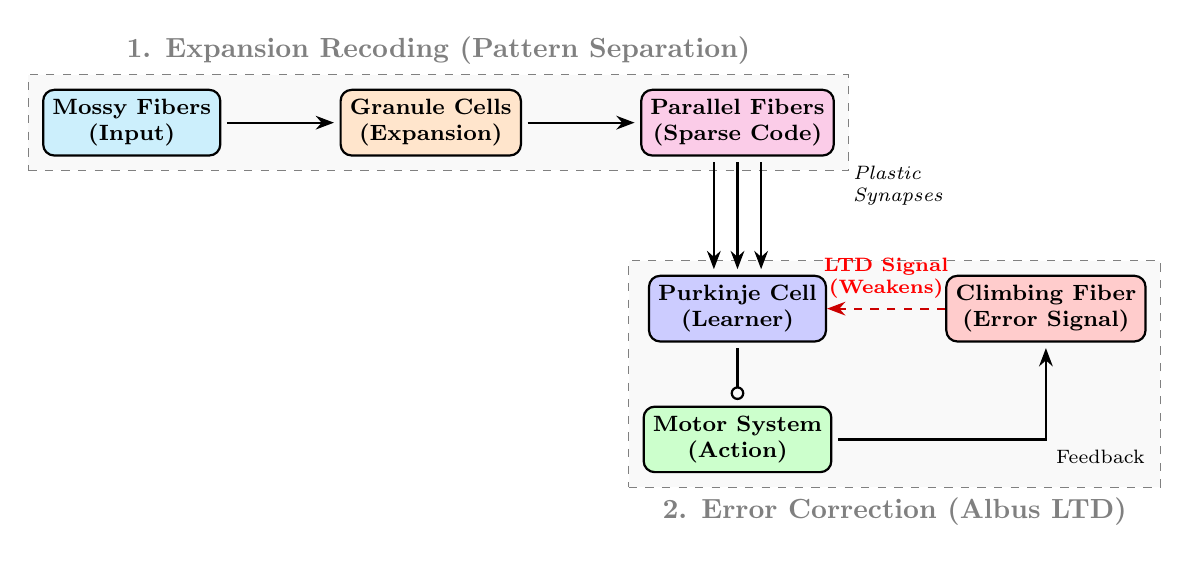
\begin{tikzpicture}[
	node distance=1.0cm and 1.5cm, % Tighter spacing for slide fit
	thick,
	>=Stealth,
	scale=1.0, transform shape, % Scale down to fit
	% Style for Nodes
	object/.style={
		rectangle,
		rounded corners,
		draw=black,
		minimum width=2.2cm,
		minimum height=0.8cm,
		align=center,
		font=\bfseries\footnotesize
	},
	% Specific Node Styles
	input/.style={object, fill=cyan!20},    % Mossy Fibers
	layer/.style={object, fill=orange!20},  % Granule Cells
	context/.style={object, fill=magenta!20},% Parallel Fibers
	output/.style={object, fill=blue!20},   % Purkinje Cell
	teacher/.style={object, fill=red!20},   % Climbing Fiber
	outcome/.style={object, fill=green!20}, % Motor Output/Error
	% Arrow Styles
	connection/.style={->, shorten >=2pt, shorten <=2pt},
	plasticity/.style={->, dashed, color=red!80!black, thick},
	inhibition/.style={-{Circle[open]}, shorten >=2pt, shorten <=2pt}
	]
	
	% --- TOP LAYER: PATTERN SEPARATION ---
	
	% Input Stage
	\node[input] (MF) {Mossy Fibers\\(Input)};
	
	% Expansion Stage
	\node[layer, right=of MF] (GC) {Granule Cells\\(Expansion)};
	
	% Context Stage
	\node[context, right=of GC] (PF) {Parallel Fibers\\(Sparse Code)};
	
	% --- BOTTOM LAYER: ERROR CORRECTION ---
	
	% Output Stage (Purkinje)
	\node[output, below=1.5cm of PF] (PC) {Purkinje Cell\\(Learner)};
	
	% Teacher/Error Stage
	\node[teacher, right=of PC] (CF) {Climbing Fiber\\(Error Signal)};
	
	% Outcome Stage
	\node[outcome, below=0.8cm of PC] (Motor) {Motor System\\(Action)};
	
	% --- CONNECTIONS ---
	
	% Feedforward Path
	\draw[connection] (MF) -- (GC);
	\draw[connection] (GC) -- (PF);
	
	% Synaptic Connection (Plasticity Site)
	% Drawing multiple connections to represent the many PFs
	\foreach \x in {-0.3, 0, 0.3} {
		\draw[connection] ($(PF.south) + (\x, 0)$) -- ($(PC.north) + (\x, 0)$);
	}
	% Label for plastic synapses
	\node[right=0.1cm of PF, yshift=-0.8cm, font=\scriptsize\itshape, align=left] (SynapseLabel) {Plastic\\Synapses};
	
	% Output Path (Inhibitory)
	\draw[inhibition] (PC) -- (Motor);
	
	% Error Loop
	% Motor error drives Climbing Fiber
	\draw[connection] (Motor.east) -| node[midway, below right, font=\scriptsize] {Feedback} (CF.south);
	
	% Teaching Signal (Albus LTD Rule)
	\draw[plasticity] (CF.west) -- node[midway, above, align=center, font=\scriptsize\bfseries, color=red] {LTD Signal\\(Weakens)} (PC.east);
	
	% --- GROUPING LABELS ---
	
	% Expansion Recoding Box
	\begin{scope}[on background layer]
		\node[draw=gray, dashed, fill=gray!5, inner sep=5pt, fit=(MF) (GC) (PF), label={[gray]above:\textbf{1. Expansion Recoding (Pattern Separation)}}] {};
	\end{scope}
	
	% Error Correction Box
	\begin{scope}[on background layer]
		\node[draw=gray, dashed, fill=gray!5, inner sep=5pt, fit=(PC) (CF) (Motor), label={[gray]below:\textbf{2. Error Correction (Albus LTD)}}] {};
	\end{scope}
	
\end{tikzpicture}

	\end{frame}
	
	\begin{frame}
		\frametitle{The neural manifolds proposal}
		\begin{itemize}
			\item Marr-Albus theory has been validated in low-dimensional motor tasks \parencite{bucknerOrganizationHumanCerebellum2011}
			\item In those tasks the `state' is simple: join angle, velocity, retinal slip
			\item We lack a rigorous way to model the state sapce of cognitive tasks, which are high-dimensional and abstract (value, risk, conflict, etc.)
			\item We propose a topological manifold constructed by the Granule Layer
		\end{itemize}
	\end{frame}
	
	\begin{frame}
		\frametitle{The neural manifolds proposal}
\begin{figure}
	\centering
	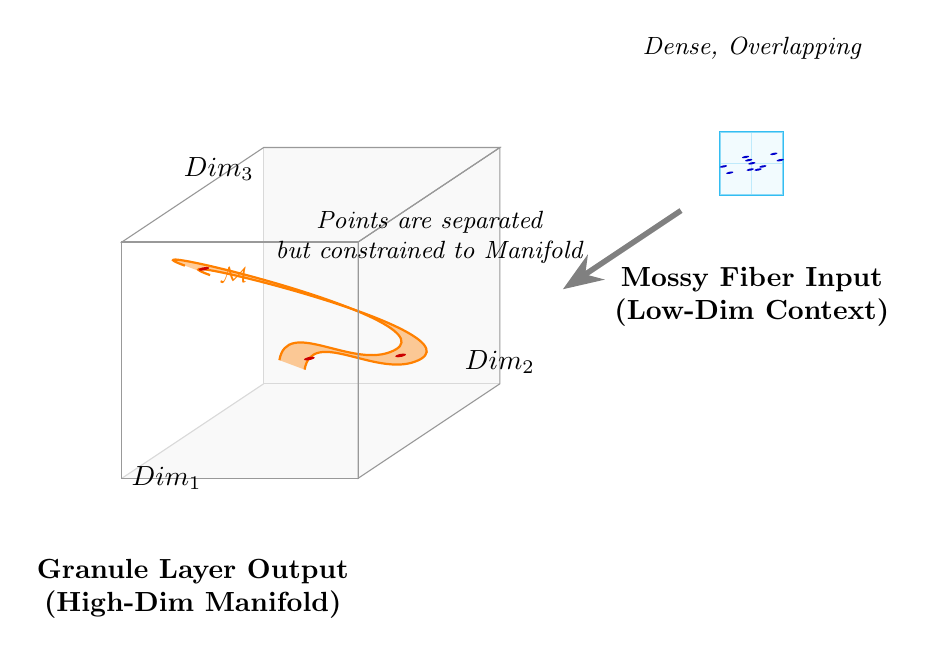
\begin{tikzpicture}[
		scale=1.0,
		% Define a custom 3D coordinate system manually for stability
		x={(-0.6cm,-0.4cm)}, y={(1cm,0cm)}, z={(0cm,1cm)},
		>={Stealth[scale=1.2]},
		node distance=3cm
		]
		
		% --- 1. LOW-DIMENSIONAL INPUT SPACE (Mossy Fibers) ---
		% Drawn as a small 2D plane with dense points
		% We shift it to the left in "visual" coordinates, not 3D logic coordinates for simplicity in placement
		\begin{scope}[shift={(-5,2)}] 
			% We'll draw a simple 2D grid here representing the input space
			\draw[cyan!40, thin] (-1,-1) grid (1,1);
			\draw[cyan!80, thick] (-1,-1) rectangle (1,1);
			\fill[cyan!10, opacity=0.5] (-1,-1) rectangle (1,1);
			
			% Dense Points (Contexts) - Clumped together
			\foreach \x/\y in {0.1/0.2, 0.2/0.1, -0.1/0.3, 0.0/0.0, 0.3/-0.1, -0.2/-0.2, 0.1/-0.3, -0.3/0.1, 0.2/0.2, -0.1/-0.1} {
				\fill[blue!80!black] (\x, \y) circle (0.04);
			}
			
			% Label
			\node[below=1.2cm, align=center, font=\bfseries] {Mossy Fiber Input\\(Low-Dim Context)};
			\node[above=1.2cm, font=\small\itshape] {Dense, Overlapping};
		\end{scope}
		
		
		% --- 2. THE TRANSFORMATION ARROW ---
		% Connecting the 2D plane to the 3D cube
		\draw[->, line width=2pt, color=gray] (-3.5, 2) -- (-1, 2) node[midway, above, font=\small\bfseries] {};
		
		
		% --- 3. HIGH-DIMENSIONAL FEATURE SPACE (Granule Layer) ---
		% Drawn as a large 3D cube at the origin of our 3D system
		\begin{scope}[shift={(2,0,0)}]
			
			% Define Cube Vertices
			\coordinate (O) at (0,0,0);
			\coordinate (X) at (3,0,0);
			\coordinate (Y) at (0,3,0);
			\coordinate (Z) at (0,0,3);
			\coordinate (XY) at (3,3,0);
			\coordinate (XZ) at (3,0,3);
			\coordinate (YZ) at (0,3,3);
			\coordinate (XYZ) at (3,3,3);
			
			% Draw Back Faces (behind everything)
			\fill[gray!5] (O) -- (Y) -- (YZ) -- (Z) -- cycle; % Left Back
			\fill[gray!5] (O) -- (X) -- (XY) -- (Y) -- cycle; % Bottom/Back? Depends on view.
			
			% Draw Edges (Back)
			\draw[gray!30] (O) -- (X);
			\draw[gray!30] (O) -- (Y);
			\draw[gray!30] (O) -- (Z);
			
			% --- THE MANIFOLD (A curved surface inside the cube) ---
			% A ribbon twisting through 3D space
			\fill[orange, opacity=0.4] 
			(0.5, 0.5, 0.5) to[out=80, in=200] 
			(1.5, 2.5, 1.0) to[out=20, in=160] 
			(2.5, 0.5, 2.5) -- 
			(2.8, 1.0, 2.5) to[out=160, in=20] 
			(1.8, 3.0, 1.0) to[out=200, in=80] 
			(0.8, 1.0, 0.5) -- cycle;
			
			% Draw lines on the manifold to show structure
			\draw[orange, thick] (0.5, 0.5, 0.5) to[out=80, in=200] (1.5, 2.5, 1.0) to[out=20, in=160] (2.5, 0.5, 2.5);
			\draw[orange, thick] (0.8, 1.0, 0.5) to[out=80, in=200] (1.8, 3.0, 1.0) to[out=20, in=160] (2.8, 1.0, 2.5);
			
			% Sparse Points ON the Manifold (Separated)
			% Manually placing points that look like they are on the ribbon
			\fill[red!80!black] (0.7, 1.0, 0.6) circle (0.06);
			\fill[red!80!black] (1.6, 2.7, 1.0) circle (0.06);
			\fill[red!80!black] (2.6, 0.8, 2.5) circle (0.06);
			
			% Draw Front Faces (Edges only)
			\draw[gray!80] (X) -- (XY) -- (XYZ) -- (XZ) -- cycle;
			\draw[gray!80] (Y) -- (XY) -- (XYZ) -- (YZ) -- cycle;
			\draw[gray!80] (Z) -- (XZ) -- (XYZ) -- (YZ) -- cycle;
			
			% Axis labels
			\node[right] at (3,0,0) {$Dim_1$};
			\node[above] at (0,3,0) {$Dim_2$};
			\node[below left] at (0,0,3) {$Dim_3$};
			
			% Labels
			\node[below=1.5cm, align=center, font=\bfseries] at (1.5, 0, 0) {Granule Layer Output\\(High-Dim Manifold)};
			\node[above=0.5cm, font=\small\itshape, align=center] at (1.5,3,1.5) {Points are separated\\but constrained to Manifold};
			
			% Annotation for Manifold
			\node[orange!100!black, font=\bfseries\footnotesize, anchor=west] at (2.8, 1.0, 2.5) {$\mathcal{M}$};
			
		\end{scope}
		
	\end{tikzpicture}
	\caption{Conceptual Visualization of Expansion Recoding as Manifold Embedding. The dense, overlapping input from Mossy Fibers (left) is projected via $f_{expand}$ into a high-dimensional feature space (Granule Layer, right). The activity patterns are not random; they are constrained to a lower-dimensional \textbf{Neural Manifold} ($\mathcal{M}$, orange surface). While globally complex, the manifold is locally structured, enabling pattern separation (red points are distant) while preserving topology for interpolation.}
\end{figure}
	\end{frame}
	
	\begin{frame}
		\frametitle{A Category-theoretic framework}
		How to derive more rigorously that the biological function between Mossy Fiber and the Granule Layer is the generation of this topological manifold? 
		\begin{itemize}
			\item We turn to Category theory for a mathematical framework to analyze \textbf{structure preservation}
			\item Allows us to make a formal comparison between two systems by observing the underlying relationships rather than the internal details
			\item The result is the capability to determine if two systems are functionally isomorphic, that is, if a function is preserved in a system it is also preserved in the other one
			\item Objective: validate a category isomorphim to inform a predictive model of cerebellum function in economic decision tasks
			\item Hypothesis: cerebellum performs expasion recording and error correction in economic decision tasks
		\end{itemize}
	\end{frame}
	
	\begin{frame}
		\frametitle{Mapping Cerebellar circuits to computational primitives}
	\centering
	Category $\mathcal{C}_{Bio}$: Functional Decomposition
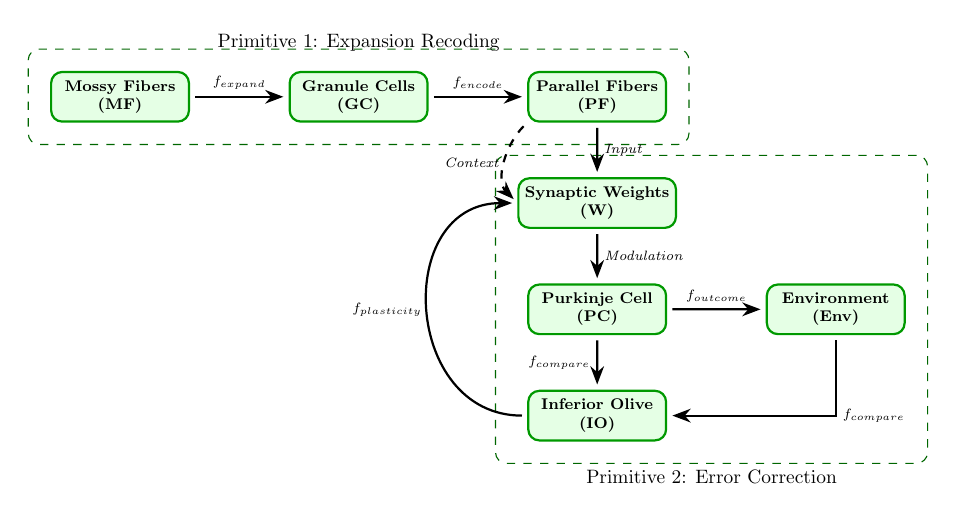
\begin{tikzpicture}[
	node distance=1.0cm and 1.8cm, % Tighter Vertical and Horizontal spacing
	thick,
	>=Stealth,
	scale=0.7, transform shape, % Scaling for slide fit
	% Style for the "Objects" (Nodes)
	object/.style={
		rectangle,
		rounded corners,
		draw=green!60!black,
		fill=green!10,
		minimum width=2.5cm,
		minimum height=0.9cm,
		align=center,
		font=\bfseries\footnotesize
	},
	% Style for "Morphisms" (Arrows)
	morphism/.style={
		->,
		shorten >=2pt,
		shorten <=2pt,
		font=\scriptsize\itshape
	},
	% Style for grouping boxes
	group/.style={
		draw=green!40!black,
		dashed,
		inner sep=8pt,
		rounded corners,
		font=\bfseries\small\color{green!40!black}
	}
	]
	
	% --- TITLE (Removed from within TikZ to use Beamer Frame Title) ---
	
	% --- NODES (OBJECTS) ---
	
	% Primitive 1: Expansion Recoding
	\node[object] (MF) {Mossy Fibers\\(MF)};
	\node[object, right=of MF] (GC) {Granule Cells\\(GC)};
	\node[object, right=of GC] (PF) {Parallel Fibers\\(PF)};
	
	% Primitive 2: Error Correction
	
	% Synaptic Weights (W) is conceptually between PF and PC
	\node[object, below=1.0cm of PF] (W) {Synaptic Weights\\(W)};
	
	% Purkinje Cell (PC)
	\node[object, below=1.0cm of W] (PC) {Purkinje Cell\\(PC)};
	
	% Environment (Env)
	\node[object, right=of PC] (Env) {Environment\\(Env)};
	
	% Inferior Olive (IO)
	\node[object, below=1.0cm of PC] (IO) {Inferior Olive\\(IO)};
	
	% --- EDGES (MORPHISMS) ---
	
	% Expansion Flow
	\draw[morphism] (MF) -- node[midway, above] {$f_{expand}$} (GC);
	\draw[morphism] (GC) -- node[midway, above] {$f_{encode}$} (PF);
	
	% Connection to Weights/PC
	\draw[morphism] (PF) -- node[midway, right] {Input} (W);
	\draw[morphism] (W) -- node[midway, right] {Modulation} (PC);
	
	% Action/Outcome
	\draw[morphism] (PC) -- node[midway, above] {$f_{outcome}$} (Env);
	
	% Feedback Loop
	\draw[morphism] (Env) |- node[midway, right] {$f_{compare}$} (IO);     % Sensory Error
	\draw[morphism] (PC) -- node[midway, left] {$f_{compare}$} (IO);      % Prediction/Inhibition
	
	% Plasticity (LTD)
	% IO -> W (long curved arrow)
	\draw[morphism] (IO.west) to[out=180, in=180, looseness=1.5] node[midway, left] {$f_{plasticity}$} (W.west);
	
	% Context for Plasticity (Eligibility Trace)
	% PF -> W (dashed dependency)
	\draw[->, dashed, shorten >=2pt, shorten <=2pt, font=\scriptsize\itshape] (PF.south west) to[out=225, in=135] node[midway, left] {Context} (W.west);
	
	% --- GROUPING BOXES (HIGHLIGHTS) ---
	
	% Primitive 1: Expansion Recoding
	\begin{scope}[on background layer]
		\node[group, fit=(MF) (GC) (PF), label={[label distance=-5pt]above:Primitive 1: Expansion Recoding}] (Group1) {};
	\end{scope}
	
	% Primitive 2: Error Correction
	\begin{scope}[on background layer]
		% We fit PC, W, Env, IO. The label is placed below.
		\node[group, fit=(PC) (W) (Env) (IO), label={[label distance=0pt]below:Primitive 2: Error Correction}] (Group2) {};
	\end{scope}
	
\end{tikzpicture}

	\end{frame}
	
	\begin{frame}
		\frametitle{Mapping Cerebellar circuits to computational primitives}
		Now to validate $\mathcal{C}_{Bio}$:
		\begin{itemize}
			\item Segment category morphisms pair-wise
			\item For each morphism perform a systematic review to determine morphism specification
			\item If both primitives hold after systematic review, then we have a theoretical validation of the category, that is, we validate its structure
		\end{itemize}
	\end{frame}
	
	\begin{frame}
		After morphism validation, we introduce `functors', which is the structure preserving mapping between $\mathcal{C}_{Bio}$ and $\mathcal{C}_{Comp}$ that represent our attempt to model the biological functions.
		$$\mathcal{F}(MF) \cong PC \text{\ (Raw EEG data)}$$
		$$\mathcal{F}(GC) \cong TF \text{\ (Topological features)}$$
		$$\vdots$$
		
	\end{frame}
	
	\begin{frame}
		\centering
		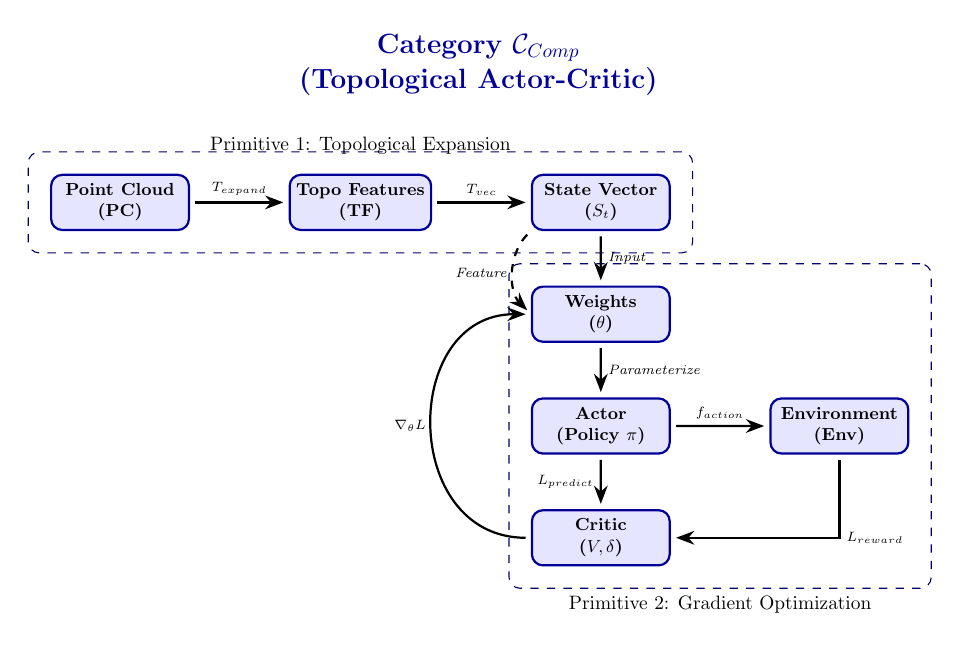
\begin{tikzpicture}[
			node distance=1.2cm and 1.8cm, % Vertical and Horizontal spacing
			thick,
			>=Stealth,
			scale=0.7, transform shape,
			% Style for the "Objects" (Nodes)
			object/.style={
				rectangle,
				rounded corners,
				draw=blue!60!black,
				fill=blue!10,
				minimum width=2.5cm,
				minimum height=1.0cm,
				align=center,
				font=\bfseries\small
			},
			% Style for "Morphisms" (Arrows)
			morphism/.style={
				->,
				shorten >=2pt,
				shorten <=2pt,
				font=\scriptsize\itshape
			},
			% Style for grouping boxes
			group/.style={
				draw=blue!40!black,
				dashed,
				inner sep=8pt,
				rounded corners,
				font=\bfseries\small\color{blue!40!black}
			}
			]
			
			% --- TITLE ---
			\node[align=center, font=\Large\bfseries\color{blue!60!black}] at (6.5, 2.5) {Category $\mathcal{C}_{Comp}$\\(Topological Actor-Critic)};
			
			% --- NODES (OBJECTS) ---
			
			% Primitive 1: Topological Expansion
			\node[object] (PC) {Point Cloud\\(PC)};
			\node[object, right=of PC] (TF) {Topo Features\\(TF)};
			\node[object, right=of TF] (SV) {State Vector\\($S_t$)};
			
			% Primitive 2: Gradient Optimization
			
			% Weights (Theta) is conceptually between SV and Actor
			\node[object, below=1.0cm of SV] (Theta) {Weights\\($\theta$)};
			
			% Actor (Policy)
			\node[object, below=1.0cm of Theta] (Actor) {Actor\\(Policy $\pi$)};
			
			% Environment (Env)
			\node[object, right=of Actor] (Env) {Environment\\(Env)};
			
			% Critic (Value/Error)
			\node[object, below=1.0cm of Actor] (Critic) {Critic\\($V, \delta$)};
			
			% --- EDGES (MORPHISMS) ---
			
			% Expansion Flow (TDA Pipeline)
			\draw[morphism] (PC) -- node[midway, above] {$T_{expand}$} (TF);
			\draw[morphism] (TF) -- node[midway, above] {$T_{vec}$} (SV);
			
			% Connection to Weights/Actor
			\draw[morphism] (SV) -- node[midway, right] {Input} (Theta);
			\draw[morphism] (Theta) -- node[midway, right] {Parameterize} (Actor);
			
			% Action/Outcome
			\draw[morphism] (Actor) -- node[midway, above] {$f_{action}$} (Env);
			
			% Feedback Loop (Loss Calculation)
			\draw[morphism] (Env) |- node[midway, right] {$L_{reward}$} (Critic);     % Reward Signal
			\draw[morphism] (Actor) -- node[midway, left] {$L_{predict}$} (Critic);    % Value Prediction
			
			% Plasticity (Gradient Descent)
			% Critic -> Theta (long curved arrow)
			\draw[morphism] (Critic.west) to[out=180, in=180, looseness=1.5] node[midway, left] {$\nabla_\theta L$} (Theta.west);
			
			% Context for Gradient (Eligibility Trace)
			% SV -> Theta (dashed dependency)
			\draw[->, dashed, shorten >=2pt, shorten <=2pt, font=\scriptsize\itshape] (SV.south west) to[out=225, in=135] node[midway, left] {Feature} (Theta.west);
			
			% --- GROUPING BOXES (HIGHLIGHTS) ---
			
			% Primitive 1: Topological Expansion
			\begin{scope}[on background layer]
				\node[group, fit=(PC) (TF) (SV), label={[label distance=-5pt]above:Primitive 1: Topological Expansion}] (Group1) {};
			\end{scope}
			
			% Primitive 2: Gradient Optimization
			\begin{scope}[on background layer]
				% We fit Actor, Theta, Env, Critic. The label is placed below.
				\node[group, fit=(Actor) (Theta) (Env) (Critic), label={[label distance=0pt]below:Primitive 2: Gradient Optimization}] (Group2) {};
			\end{scope}
			
		\end{tikzpicture}
	\end{frame}
	
	\begin{frame}
		\frametitle{Validating the functors validates the isomorphism}
		Each morphism generates a prediction, the functor is validated if the morphism in $\mathcal{C}_{Comp}$ behaves maintaining the same `metric space' (the same ranking after transformations). For example for the functor $\mathcal{F}(GC) \cong TF$:
		$$d_{GC}(f(x), f(y)) >> d_{MF}(x, y)$$
		Is `metric space' prediction, and the validation can be statistically tested with:
		$$\frac{d_{PI}(T(u), T(v))}{d_{PC}(u, v)} > 1$$
		With $PI$ being the persistence image, and $PC$ the Purkinje cell output (behavioral space)
	\end{frame}

	\begin{frame}
		\frametitle{Representational similarity analysis}
		To get the empirical support for the categorical construction. We propose a simple 2-armed bandit with rewards determined by gaussian random walks. With representational similarity matrices:
		$$RSM_{neural} \rightarrow v \in \mathcal{R}^{320} \ \text(64 \ channels \ x \ 5 \ frequency \ bands)$$
		$$RSM_{raw} \rightarrow v \in \{win, loss\}$$
		$$RSM_{model} \rightarrow PI$$
	\end{frame}
	
	\begin{frame}
		\frametitle{Representational similarity analysis}
		Then the statistical tests are:
		$$spearmanCor(RSM_{neural}, RSM_{model}) > 0$$
		$$Ratio_{neural} = \frac{d_{neural}(v_{i}, v_{j})}{d_{raw}(v_{i}, v_{j})}$$
		$$Ratio_{model} = \frac{d_{model}(v_{i}, v_{j})}{d_{raw}(v_{i}, v_{j})}$$
		$$Ratio_{model} > 1 \land Ratio_{model} \approx Ratio_{neural}$$
	\end{frame}
	
	\begin{frame}
		\frametitle{Building the complete category-theoretic model}
		The reinforcement learning actor-critic is built from the category isomorphism as:
		$$\Delta \theta \propto \alpha \cdot \delta_{t} \cdot \nabla_{\theta} \log \pi (A_{t}|S_{t})$$
		Which would allow us to perform a cerebellar zone perturbation using TMS and contrasting that to model prediction in both biological and behavioral domains simultaneously, and within a clearly tractable framework (the category isomorphism)
	\end{frame}
	
\end{document}